\section{Prestudy}\label{prestudy} This project is one that requires quite a lot of prestudy before we can begin coding or even designing the architecture. Since the customer wanted us to implement existing technologies, such as Glassfish, WSO2, SAML etc. we need to spend some time researching those technologies to figure out what to use, and how to use it. The following sections will describe the overall architecture of how we, at this point in time, imagine our system will be like. 

        \begin{figure}[htb]
            \centering
            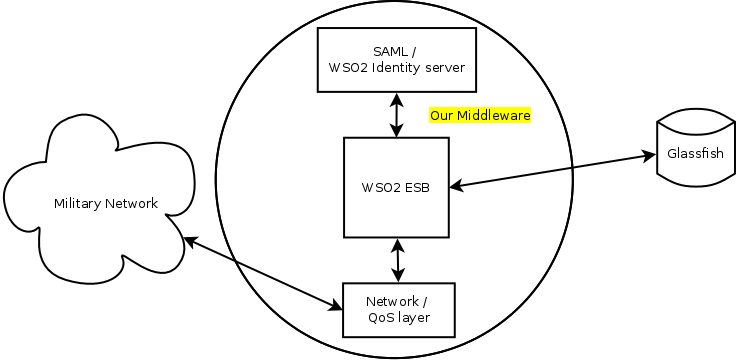
\includegraphics[scale=0.4]{birdarch}
            \caption{Bird view of the thought of architecture.}
            \label{fig:birdarch}
        \end{figure}

    \subsection{Server side Architecture}\label{serversidearch} [The architecture of the server side module we are to create.] 
    
        The server side architecture consists of several components, the WSO2 ESB, the WSO2 Identity Server, the Tactical Router and the GlassFish server. All of these components are already available, so what we will have to make is mediators in the ESB.

        Before the client can request a web service it has to have an identification. To get an ID-token it has to contact the Identity Server using the ESB as a proxy (Fig.\ref{fig:serverside}-1). Then the client can request a web service from the ESB. Several things will then happen in the ESB. First the request message is sent to the SAML mediator (Fig.\ref{fig:serverside}-2), this mediator contacts the Identity Server to validate the clients ID-token (Fig.\ref{fig:serverside}-3). If the token is validated and the client is supposed to have access to the requested service the message is passed on to the GlassFish proxies (Fig.\ref{fig:serverside}-4), otherwise it is dropped. The ESB acting as a proxy will then send the request along to the requested service on the GlassFish server (Fig.\ref{fig:serverside}-5).

        \begin{figure}[htb]
            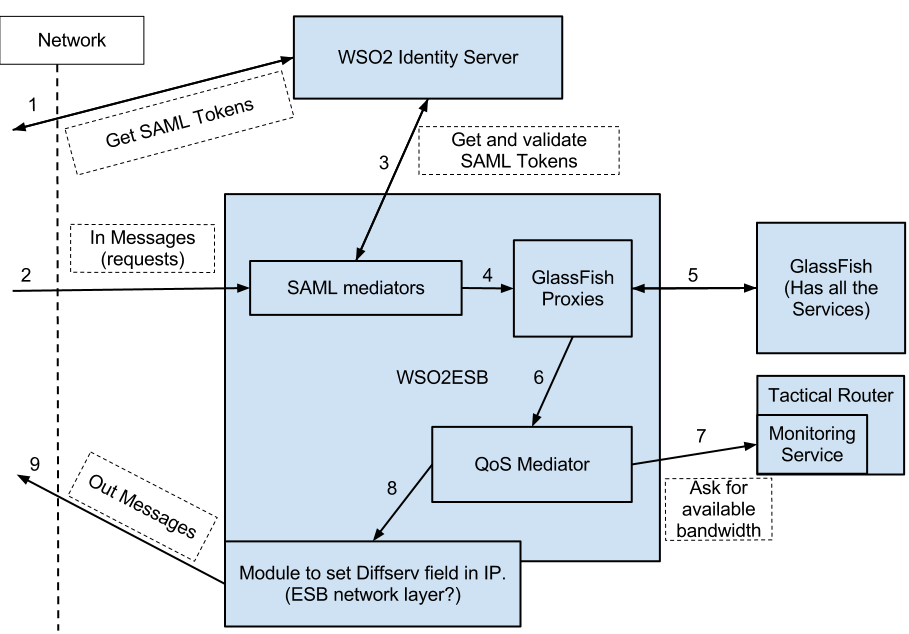
\includegraphics[scale=0.5]{Serversidearchitecture}
            \caption{The Server side Architecture}
            \label{fig:serverside}
        \end{figure}

        When the request is received at the service, it will probably start sending some data to the client. This is also done through the ESB. First the message is sent to the QoS mediator (Fig.\ref{fig:serverside}-6). This mediator will first look at the role, or identity, of the client and the service requested, and use this information to assign a priority to the connection. Then the Tactical Router is contacted for bandwidth information (Fig.\ref{fig:serverside}-7), which is used together with the priority to determine whether the message should be sent right away or held back until some higher priority message is finished sending.

        Either in the QoS mediator, in the ESB’s network layer, or after that, the Diffserv (ToS) field of the IP header will have to be set (Fig.\ref{fig:serverside}-8) before the message is sent to the client (Fig.\ref{fig:serverside}-9). This field is used by the routers in the network to prioritize packet sending. This step is quite important to the whole procedure as this is one of the few requirements the customer has given us, as such this step can not be dropped from the final product.
 
    \subsection{Client side Architecture}\label{clientsidearch} [The architecture of the client side module we are goint to create.] 
    
        The client-side architecture will be composed of altered (already existing) client software, the OpenSAML library as well as our client library implementation.
        
        \begin{figure}[htb]
            \centering
            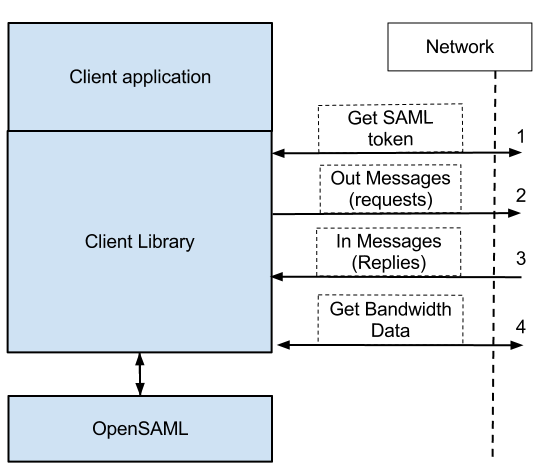
\includegraphics[scale=0.5]{Client-sideArchitechture}
            \caption{The Client side Architecture}
            \label{fig:clientside}
        \end{figure}
 
        Before the client library can ask for the data the client needs to get a SAML authentication token from the identity server (Fig.\ref{fig:clientside}-1). The communication here will most likely be handled by our library, but the SAML packages will be created and analyzed by the OpenSAML library. 

        The client library then sends the request from the client to the server (Fig.\ref{fig:clientside}-2), appending the SAML token to the package as well as adding some metadata in the SOAP header related to the client role and setting the TOS field of the package to a default value.

        The reply from the server is examined by our client library for the metadata the server has embedded in the SOAP header, relevant metadata is stored for future communication and the package is passed to the client application (Fig.\ref{fig:clientside}-3).

        When new communication is initiated after this first connection is made the client should, if everything went as expected, have the necessary information to prioritize new messages. This means that the client can now take quite an informed decision about how it should prioritize messages, but in order to do this to the best of it’s abilities it also has to take into consideration available bandwidth (Fig.\ref{fig:clientside}-4).
    
           
    \subsection{Alternative solutions}\label{alternativesolutions} [Sollutions that we have, thought about but discarded.]
    
        Since this is only the preliminary report we have not yet decided on a final solution to the task at hand. But we have taken some decisions which will influence alternative solutions and will lock out some possible avenues of research.

        Since you can see an outline to the architecture in (\ref{prestudy}) we will instead use this section to outline some of the alternative architectures which we looked at, but rejected for the moment.

        The customer also gave us a paper\cite{soa-qos-pdf} which described a previous project they had worked on which tried to solve something quite similar to what we were tasked with. The paper described a system which were used in conjunction with Tactical routers(\ref{glossary}) to retrieve bandwidth information and to control sending of messages into this network. As the customer explained this work was not something we could directly copy as the project had not used a lot of web standards and had focused more on the tactical routers as opposed to web services. What we could take out of it however was how they throttled messages. The paper contained five methods which we could easily implement and use their result as an indication of what methods we should use to throttle or hold back messages.

        One architecture, which our customer suggested for the project, was to have a proxy in between nodes and creating a custom QoS layer which would sit in front of both the client and the services. This layer would then communicate with a SAML server for authentication, and would have to do all the message prioritization based on the same criteria as our architecture. There are several points about this architecture which would make it a good fit for us. Since the QoS layer would be identical on both client and server side it would mean less work, and more code that could be shared among components, but this freedom comes with some downsides. The first and most glaring problem encountered would be that services on the server would have to be altered to be able to communicate with this front end. Even though we were free to choose architecture ourselves, the client expressed a wish that we would not choose this model because the customer wants to use COTS(\ref{glossary}) services which would not be compatible with the new front end.

        Even though the above mentioned architecture is not the best fit for us we wanted to take some aspects of the architecture further. Since clients can easily be altered, the above mentioned solution is not applicable for server side, the solution could however be used for the clients. Having a proxy on the client side could be quite good, but because of the work involved and probable time constraints we chose not to go with this solution. On the server side however a front end is not the best solution for us. What we instead are looking into, is to use an ESB(\ref{glossary}) which would be configured together with the services and work as a proxy. Because many ESBs have integrated SAML processing we could easily take advantage of such facilities along with custom message processing, with which we would then extend the ESB to support our needs. The clients would have to point to the ESB, but this should both be trivial to do and the customer has expressed their agreement that this is satisfactory. We could eventually expand the functionality with service discovery, which then would be a good solution to the problem.

        So far we have outlined major alternative architectures which could be alternatives to our project, but there are also alternatives within our proposed solution. One such alternative is not to use a premade ESB, but rather build one ourselves. This solution was thoroughly investigated, but was eventually turned down because of the massive amount of work that had to be done, the quality of an already made ESB is much higher than we could ever achieve during this project, and lastly, the open source tools available to implement the functionality needed for SAML was not very well documented, and would take considerable time to get familiar with.

        On the client side we also have the choice of having either a HTTP proxy or writing our own custom library. Both have some advantages and disadvantages, a proxy would be better for integration with client programs, but creating this proxy or configuring and customizing an already existing solution is not trivial. On the same note, creating a library for use in client programs is easier, but this would mean that client programs would need to be altered to be usable with our middleware, which isn’t that desirable. We chose to go down the road of least resistance, as we see it currently we would have do quite a lot of research into proxies which could in the worst case scenario result in just wasted time as far as our product goes. A client library would from our perspective be easier as we would have more control, the overall design should be easier and we know that with this sort of library we can integrate OpenSAML which is a huge advantage.  
          
